\chapter{Competitividad en las últimas temporadas}

En este capítulo aplicaremos la aplicación implementada para comparar entre las cuatro últimas temporadas de la Liga BBVA, y decidir cuál de ellas es la que mayor competitividad ha tenido.\\

\section{Temporada 2011-2012}

El grafo de competitividad y el histórico de posiciones de la temporada 2011-2012 se muestra en la Figura~\ref{fig:grafo-2011-2012}.


\begin{figure}[htbp]
\centering
\subfigure[Grafo de competitividad]{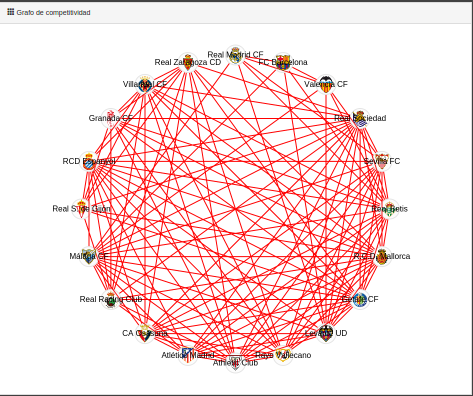
\includegraphics[width=0.5\textwidth]{imagenes/pantallazos-competitividad/2011-2012/grafo}}
\subfigure[Histórico de posiciones]{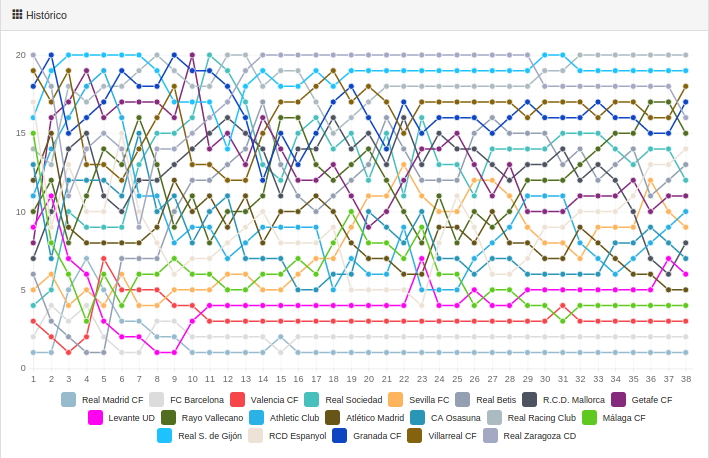
\includegraphics[width=0.5\textwidth]{imagenes/pantallazos-competitividad/2011-2012/historico}}
\caption[Competitividad de la temporada 2011-2012]{Grafo de competitividad e histórico de posiciones de la temporada 2011-2012} \label{fig:grafo-2011-2012}
\end{figure}

\clearpage

\section{Temporada 2012-2013}

El grafo de competitividad y el histórico de posiciones de la temporada 2012-2013 se muestra en la Figura~\ref{fig:grafo-2012-2013}.

\begin{figure}[htbp]
\centering
\subfigure[Grafo de competitividad]{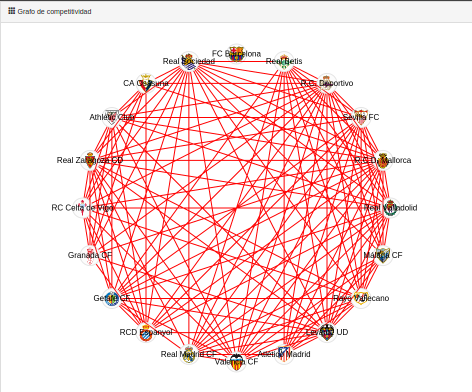
\includegraphics[width=0.5\textwidth]{imagenes/pantallazos-competitividad/2012-2013/grafo}}
\subfigure[Histórico de posiciones]{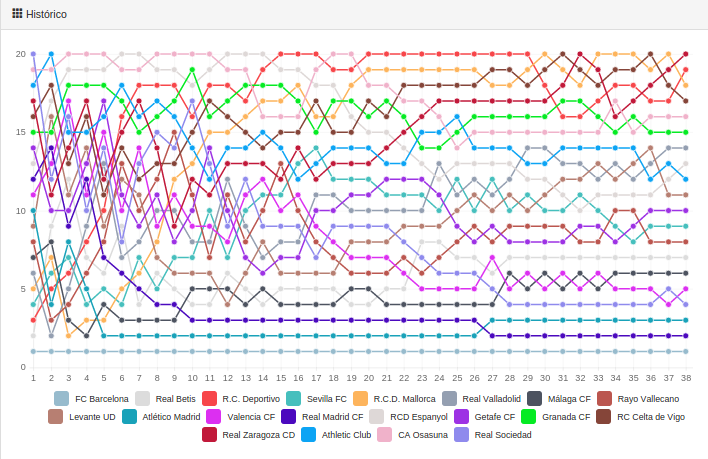
\includegraphics[width=0.5\textwidth]{imagenes/pantallazos-competitividad/2012-2013/historico}}
\caption[Competitividad de la temporada 2012-2013]{Grafo de competitividad e histórico de posiciones de la temporada 2012-2013} \label{fig:grafo-2012-2013}
\end{figure}

\clearpage

\section{Temporada 2013-2014}

El grafo de competitividad y el histórico de posiciones de la temporada 2013-2014 se muestra en la Figura~\ref{fig:grafo-2013-2014}.

\begin{figure}[htbp]
\centering
\subfigure[Grafo de competitividad]{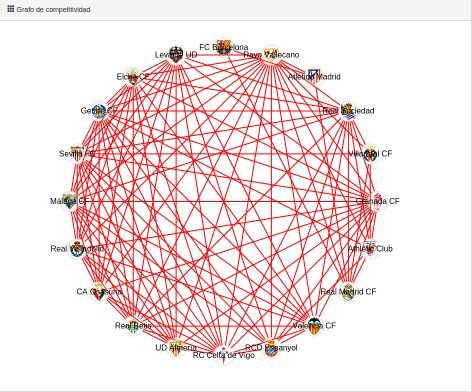
\includegraphics[width=0.5\textwidth]{imagenes/pantallazos-competitividad/2013-2014/grafo}}
\subfigure[Histórico de posiciones]{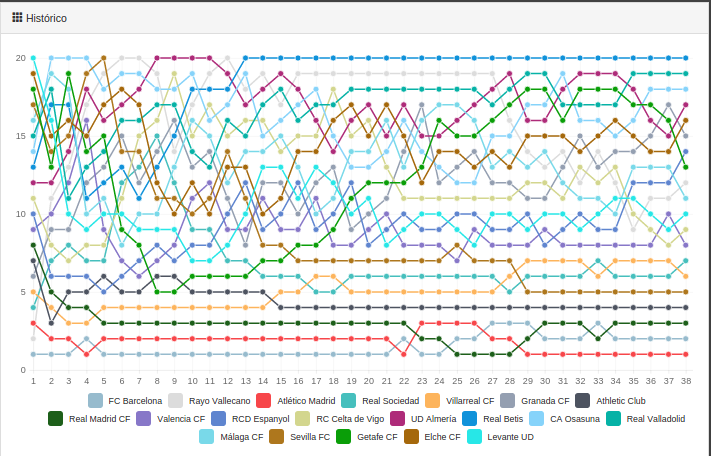
\includegraphics[width=0.5\textwidth]{imagenes/pantallazos-competitividad/2013-2014/historico}}
\caption[Competitividad de la temporada 2013-2014]{Grafo de competitividad e histórico de posiciones de la temporada 2013-2014} \label{fig:grafo-2013-2014}
\end{figure}

\clearpage

\section{Temporada 2014-2015}

El grafo de competitividad y el histórico de posiciones de la temporada 2014-2015 se muestra en la Figura~\ref{fig:grafo-2014-2015}.

\begin{figure}[htbp]
\centering
\subfigure[Grafo de competitividad]{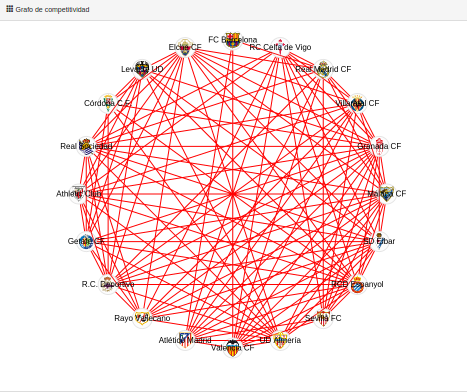
\includegraphics[width=0.5\textwidth]{imagenes/pantallazos-competitividad/2014-2015/grafo}}
\subfigure[Histórico de posiciones]{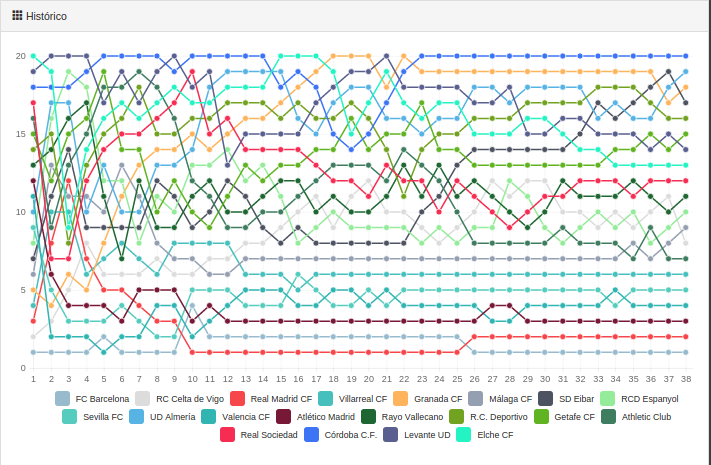
\includegraphics[width=0.5\textwidth]{imagenes/pantallazos-competitividad/2014-2015/historico}}
\caption[Competitividad de la temporada 2014-2015]{Grafo de competitividad e histórico de posiciones de la temporada 2014-2015} \label{fig:grafo-2014-2015}
\end{figure}

\clearpage

\section{Estudio de la competitividad}

Los gráficos anteriores no nos dan muchas información de qué temporadas son las más competitivas, por lo que debemos emplear las medidas de competitividad para poder comparar la competitividad. La Tabla~\ref{tbl:medidas} muestra las medidas de competitividad de cada una de las temporadas.

\begin{table}[h]
\centering
\caption[Medidas de competitividad]{Medidas de competitividad de las temporadas 2011-2012, 2012-2013, 2013-2014 y 2014-2015 de la Liga BBVA. Las medidas son fuerza media normalizada (NMS), el diámetro, la tau de Kendall, el grado medio normalizado (NMD), la longitud del camino característico (CPL) y la eficienncia.}
\label{tbl:medidas}
\begin{tabular}{@{}ccccccc@{}}
\toprule
Temporada & NMS & Diámetro & Tau de Kendall & NMD & CPL & Eficiencia \\ \midrule
2014-2015 & 0.642                    & 3        & 0.054          & 0.891                   & 2.768                              & 1.633      \\
2013-2014 & 0.594                    & 3        & 0.059          & 0.880                   & 2.9368                             & 1.573      \\
2012-2013 & 0.673                    & $\infty$ & 0.061          & 0.876                   & $\infty$                           & 1.574      \\
2011-2012 & 0.636                    & 3        & 0.066          & 0.867                   & 2.789                              & 1.626      \\ \bottomrule
\end{tabular}
\end{table}

Con respecto al diámetro del grafo de competitividad evolutivo, vemos que las temporadas 2014-2015, 2013-2014 y 2011-2012 tienen el mismo diámetro, 3, mientras que la temporada 2012-2013 tiene diámetro infinito. Esto se debe a que existen dos componentes conexas en el grafo de competitividad.\\
Por tanto, las temporadas 2014-2015, 2013-2014 y 2011-2012 son más competitivas que la temporada 2012-2013 con respecto al diámetro del grafo de competitividad evolutivo.\\

Con respecto a la fuerza media normalizada, podemos observar que el valor más alto es el relativo a la temporada 2012-2013, por lo que esta temporada es la más competitiva con respecto a esta medida, seguida de la temporada 2014-2015, 2011-2012 y 2013-2014.\\

Con respecto a la tau de Kendall evolutiva, el valor más bajo lo tiene la temporada 2014-2015, por lo que es la temporada más competitiva, seguida de las temporadas 2013-2014, 2012-2013 y 2011-2012.\\

Con respecto al grado medio normalizado, la temporada más competitiva es la 2014-2015 ya que es la que tiene el mayor valor para esta medida. Seguidamente vendrían las temporadas 2013-2014, 2012-2013 y 2011-2012.\\

Con respecto a la longitud del camino característico, la temporada más competitiva con respecto a esta medida es la temporada 2014-2015, seguida de la temporada 2011-2012, 2013-2014 y 2012-2013.\\

Por último, con respecto a la eficiencia, la temporada más competitiva es es la 2014-2015 seguida de las temporadas 2011-2012, 2013-2014 y 2012-2013.\\

Por tanto, la temporada más competitiva de las analizadas es la 2014-2105 ya que es la más competitiva en 4 de las 6 medidas (tau de Kendall, grado medio normalizado, longitud del camino característico y eficiencia), es segunda en una de ellas (fuerza media normalizada) y es primera empatada con otra tres temporadas en otra (diámetro). 
